\documentclass[../../../main.tex]{subfiles}
\begin{document}

%%%%%%%%%%%%%%%%%%%%%%%%%%%%%%%%%%%%%%%%%
%%%%%%%%%%%%%%%%%%%%%%%%%%%%%%%%%%%%%%%%%
%%%%%%%%%%%%%%%%%%%%%%%%%%%%%%%%%%%%%%%%%
\chapter{Probability as area}

With continuous values, we can think of probability as the area under a polygon plot. But this works for discrete values too, so we'll start with that, and work up to continuous values.


%%%%%%%%%%%%%%%%%%%%%%%%%%%%%%%%%%%%%%%%%
%%%%%%%%%%%%%%%%%%%%%%%%%%%%%%%%%%%%%%%%%
\section{A coin flip}

Think of a coin flip. There are two outcomes, so the chances of getting each is .5. 

Let's plot the points as a polygon:

\begin{center}
  \begin{tikzpicture}

    \draw[->] (0, 0) -- (0, 4);
    \draw (-0.1, 1) -- (0.1, 1);
    \node (ytick1) at (0, 1) [label=left:{0.25}] {};
    \draw (-0.1, 2) -- (0.1, 2);
    \node (ytick2) at (0, 2) [label=left:{.5}] {};
    \draw (-0.1, 3) -- (0.1, 3);
    \node (ytick3) at (0, 3) [label=left:{0.75}] {};

    \draw[->] (0, 0) -- (7, 0);
    \draw (2, -0.1) -- (2, 0.1);
    \node (xtick1) at (2, 0) [label=below:{heads}] {};
    \draw (4, -0.1) -- (4, 0.1);
    \node (xtick3) at (4, 0) [label=below:{tails}] {};

    \fill[color=lightgray] (0, 2) -- (6, 2) -- (6, 0) -- (0, 0) -- (0, 2);
    \draw (6, 0) -- (0, 0) -- (0, 2) -- (6, 2);
    \node[dot-point] (heads_dot) at (2, 2) {};
    \node[dot-point] (tails_dot) at (4, 2) {};
    
  \end{tikzpicture}
\end{center}

This is a uniform distribution, of course, because the two outcomes have the same probability (.5 each). The area under the line therefore makes a square. 

What is the area of this square? Well, we could measure the exact size of the square, but that's silly, because we could draw it bigger or smaller. What we are really interested is what it represents. And really, it represents all the possible outcomes of the experiment (a coin flip). 

But we know that the probabilities of all possible outcomes always adds up to 1 (or 100\%). So let's just say that the area under the line is 1.

Now, let's break up the square into two equal pieces, one to represent the probability of flipping heads, and the other to represent the probability of getting tails:

\begin{center}
  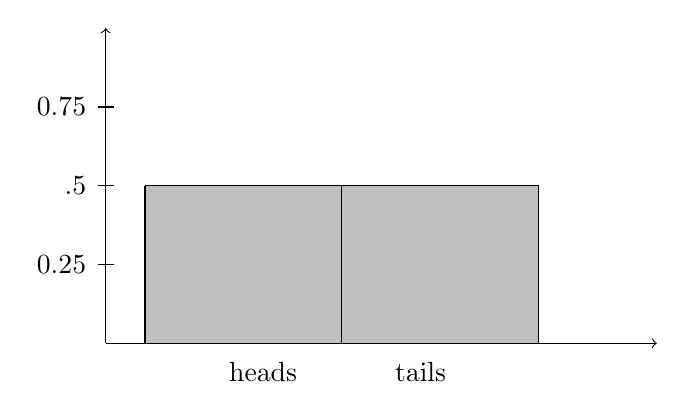
\begin{tikzpicture}

    \draw[->] (0, 0) -- (0, 4);
    \draw (-0.1, 1) -- (0.1, 1);
    \node (ytick1) at (0, 1) [label=left:{0.25}] {};
    \draw (-0.1, 2) -- (0.1, 2);
    \node (ytick2) at (0, 2) [label=left:{.5}] {};
    \draw (-0.1, 3) -- (0.1, 3);
    \node (ytick3) at (0, 3) [label=left:{0.75}] {};

    \draw[->] (0, 0) -- (7, 0);
    \node (xtick1) at (2, 0) [label=below:{heads}] {};
    \node (xtick3) at (4, 0) [label=below:{tails}] {};

    \draw[fill=lightgray] (0.5, 2) -- (5.5, 2) -- (5.5, 0) -- (0.5, 0) -- (0.5, 2);
    \draw (3, 2) -- (3, 0);

  \end{tikzpicture}
\end{center}

We can see that the area of each outcome is exactly half, or 0.5. And that makes sense. If all possibilities that could possibly happen with a coin flip add up to 1, and there are only two possible outcomes, then each outcome must be .5.

So, we can think of the \vocab{area} of each segment of the plot as the \vocab{probability} for that outcome. And indeed, the probability of each outcome is represented exactly by the area under the line. If we treat the whole square as 100\% (or 1) of the probabilities, then each segment is half of that, namely 50\% (or .5).


%%%%%%%%%%%%%%%%%%%%%%%%%%%%%%%%%%%%%%%%%
%%%%%%%%%%%%%%%%%%%%%%%%%%%%%%%%%%%%%%%%%
\section{Rolling a six-sided die}

Think of rolling a (fair) six-sided die. Again, we can plot it with a polygon plot: 

\begin{center}
  \begin{tikzpicture}

    \draw[->] (0, 0) -- (0, 4);
    \draw (-0.1, 1) -- (0.1, 1);
    \node (ytick1) at (0, 1) [label=left:{0.083}] {};
    \draw (-0.1, 2) -- (0.1, 2);
    \node (ytick2) at (0, 2) [label=left:{0.167}] {};
    \draw (-0.1, 3) -- (0.1, 3);
    \node (ytick3) at (0, 3) [label=left:{0.333}] {};

    \draw[->] (0, 0) -- (8, 0);
    \draw (1, -0.1) -- (1, 0.1);
    \node (xtick1) at (1, 0) [label=below:{1}] {};
    \draw (2, -0.1) -- (2, 0.1);
    \node (xtick2) at (2, 0) [label=below:{2}] {};
    \draw (3, -0.1) -- (3, 0.1);
    \node (xtick3) at (3, 0) [label=below:{3}] {};
    \draw (4, -0.1) -- (4, 0.1);
    \node (xtick4) at (4, 0) [label=below:{4}] {};
    \draw (5, -0.1) -- (5, 0.1);
    \node (xtick5) at (5, 0) [label=below:{5}] {};
    \draw (6, -0.1) -- (6, 0.1);
    \node (xtick6) at (6, 0) [label=below:{6}] {};

    \fill[color=lightgray] (0, 2) -- (7, 2) -- (7, 0) -- (0, 0) -- (0, 2);
    \draw (7, 0) -- (0, 0) -- (0, 2) -- (7, 2);
    \node[dot-point] (1_dot) at (1, 2) {};
    \node[dot-point] (2_dot) at (2, 2) {};
    \node[dot-point] (3_dot) at (3, 2) {};
    \node[dot-point] (4_dot) at (4, 2) {};
    \node[dot-point] (5_dot) at (5, 2) {};
    \node[dot-point] (6_dot) at (6, 2) {};
    
  \end{tikzpicture}
\end{center}

This is also a uniform distribution, so the area under the line is just a square. Again, let's say that the total area of the square is 1 (or 100\%).

And then, let's break it up into 6 equal pieces, one for each possible outcome:

\begin{center}
  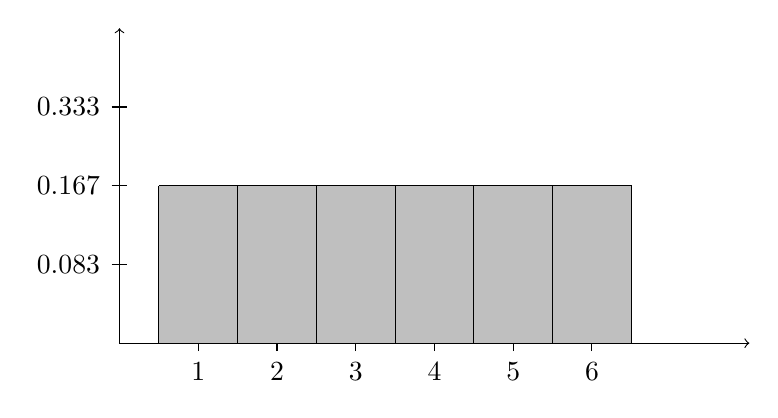
\begin{tikzpicture}

    \draw[->] (0, 0) -- (0, 4);
    \draw (-0.1, 1) -- (0.1, 1);
    \node (ytick1) at (0, 1) [label=left:{0.083}] {};
    \draw (-0.1, 2) -- (0.1, 2);
    \node (ytick2) at (0, 2) [label=left:{0.167}] {};
    \draw (-0.1, 3) -- (0.1, 3);
    \node (ytick3) at (0, 3) [label=left:{0.333}] {};

    \draw[->] (0, 0) -- (8, 0);
    \draw (1, -0.1) -- (1, 0.1);
    \node (xtick1) at (1, 0) [label=below:{1}] {};
    \draw (2, -0.1) -- (2, 0.1);
    \node (xtick2) at (2, 0) [label=below:{2}] {};
    \draw (3, -0.1) -- (3, 0.1);
    \node (xtick3) at (3, 0) [label=below:{3}] {};
    \draw (4, -0.1) -- (4, 0.1);
    \node (xtick4) at (4, 0) [label=below:{4}] {};
    \draw (5, -0.1) -- (5, 0.1);
    \node (xtick5) at (5, 0) [label=below:{5}] {};
    \draw (6, -0.1) -- (6, 0.1);
    \node (xtick6) at (6, 0) [label=below:{6}] {};

    \draw[fill=lightgray] (0.5, 2) -- (6.5, 2) -- (6.5, 0) -- (0.5, 0) -- (0.5, 2);
    \draw (1.5, 2) -- (1.5, 0);
    \draw (2.5, 2) -- (2.5, 0);
    \draw (3.5, 2) -- (3.5, 0);
    \draw (4.5, 2) -- (4.5, 0);
    \draw (5.5, 2) -- (5.5, 0);

  \end{tikzpicture}
\end{center}

We can see that the area of each outcome is exactly one-sixth, or approximately 0.167. And that makes sense. 

So again, the area of each segment exactly represents the probability of each outcome.

Notice that there are more outcomes with a die toss than there are with a coin flip, so we have more segments. And notice that as we get more segments, each segment gets narrower. The coin flip segments are fat. These segments are a little skinnier, because we have to fit more of them into the square.

The skinniness of each segment is a visual indicator of what's happening. As we get more possible outcomes, the chances of getting any particular one of them gets smaller. 

Think about tossing a dart at the square. If there are only two segments (as there were with the coin flip), it's easier to hit one of the segments, because it's pretty big. But now with six segments, it's harder to hit a particular segment with the dart, because it's skinnier. 



%%%%%%%%%%%%%%%%%%%%%%%%%%%%%%%%%%%%%%%%%
%%%%%%%%%%%%%%%%%%%%%%%%%%%%%%%%%%%%%%%%%
\section{Ranges of probabilities}

We can look at larger segments or ranges of segments of a polygon plot to tell us the probabilities of a range of values. Take the plot for rolling a (fair) six-sided die again:

\begin{center}
  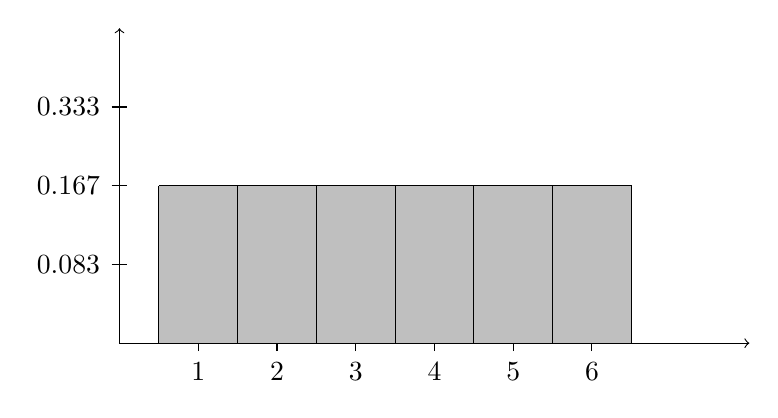
\begin{tikzpicture}

    \draw[->] (0, 0) -- (0, 4);
    \draw (-0.1, 1) -- (0.1, 1);
    \node (ytick1) at (0, 1) [label=left:{0.083}] {};
    \draw (-0.1, 2) -- (0.1, 2);
    \node (ytick2) at (0, 2) [label=left:{0.167}] {};
    \draw (-0.1, 3) -- (0.1, 3);
    \node (ytick3) at (0, 3) [label=left:{0.333}] {};

    \draw[->] (0, 0) -- (8, 0);
    \draw (1, -0.1) -- (1, 0.1);
    \node (xtick1) at (1, 0) [label=below:{1}] {};
    \draw (2, -0.1) -- (2, 0.1);
    \node (xtick2) at (2, 0) [label=below:{2}] {};
    \draw (3, -0.1) -- (3, 0.1);
    \node (xtick3) at (3, 0) [label=below:{3}] {};
    \draw (4, -0.1) -- (4, 0.1);
    \node (xtick4) at (4, 0) [label=below:{4}] {};
    \draw (5, -0.1) -- (5, 0.1);
    \node (xtick5) at (5, 0) [label=below:{5}] {};
    \draw (6, -0.1) -- (6, 0.1);
    \node (xtick6) at (6, 0) [label=below:{6}] {};

    \draw[fill=lightgray] (0.5, 2) -- (6.5, 2) -- (6.5, 0) -- (0.5, 0) -- (0.5, 2);
    \draw (1.5, 2) -- (1.5, 0);
    \draw (2.5, 2) -- (2.5, 0);
    \draw (3.5, 2) -- (3.5, 0);
    \draw (4.5, 2) -- (4.5, 0);
    \draw (5.5, 2) -- (5.5, 0);

  \end{tikzpicture}
\end{center}

There are six segments, each one representing exactly the probability of a particular outcome.

What is the probability of rolling a 2? It is exactly one-sixth, or 0.167, because that's the area of the segment that represents rolling a 2:

\begin{center}
  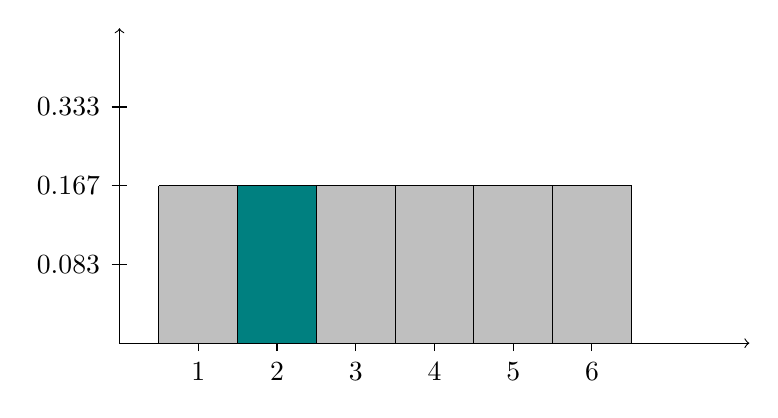
\begin{tikzpicture}

    \draw[->] (0, 0) -- (0, 4);
    \draw (-0.1, 1) -- (0.1, 1);
    \node (ytick1) at (0, 1) [label=left:{0.083}] {};
    \draw (-0.1, 2) -- (0.1, 2);
    \node (ytick2) at (0, 2) [label=left:{0.167}] {};
    \draw (-0.1, 3) -- (0.1, 3);
    \node (ytick3) at (0, 3) [label=left:{0.333}] {};

    \draw[->] (0, 0) -- (8, 0);
    \draw (1, -0.1) -- (1, 0.1);
    \node (xtick1) at (1, 0) [label=below:{1}] {};
    \draw (2, -0.1) -- (2, 0.1);
    \node (xtick2) at (2, 0) [label=below:{2}] {};
    \draw (3, -0.1) -- (3, 0.1);
    \node (xtick3) at (3, 0) [label=below:{3}] {};
    \draw (4, -0.1) -- (4, 0.1);
    \node (xtick4) at (4, 0) [label=below:{4}] {};
    \draw (5, -0.1) -- (5, 0.1);
    \node (xtick5) at (5, 0) [label=below:{5}] {};
    \draw (6, -0.1) -- (6, 0.1);
    \node (xtick6) at (6, 0) [label=below:{6}] {};

    \draw[fill=lightgray] (0.5, 2) -- (6.5, 2) -- (6.5, 0) -- (0.5, 0) -- (0.5, 2);
    \draw (1.5, 2) -- (1.5, 0);
    \draw[fill=teal] (1.5, 2) -- (2.5, 2) -- (2.5, 0) -- (1.5, 0) -- (1.5, 2);
    \draw (3.5, 2) -- (3.5, 0);
    \draw (4.5, 2) -- (4.5, 0);
    \draw (5.5, 2) -- (5.5, 0);

  \end{tikzpicture}
\end{center}

What is the probabliity of rolling a 2 or a 4? It's exactly two-sixths, or 0.334, because that's the area of the two segments together:

\begin{center}
  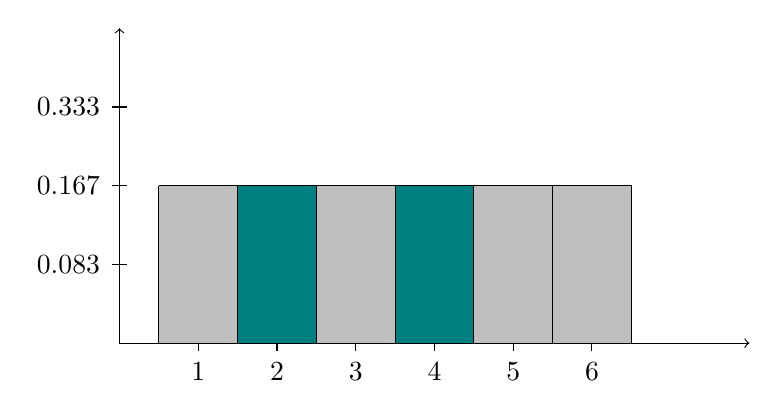
\begin{tikzpicture}

    \draw[->] (0, 0) -- (0, 4);
    \draw (-0.1, 1) -- (0.1, 1);
    \node (ytick1) at (0, 1) [label=left:{0.083}] {};
    \draw (-0.1, 2) -- (0.1, 2);
    \node (ytick2) at (0, 2) [label=left:{0.167}] {};
    \draw (-0.1, 3) -- (0.1, 3);
    \node (ytick3) at (0, 3) [label=left:{0.333}] {};

    \draw[->] (0, 0) -- (8, 0);
    \draw (1, -0.1) -- (1, 0.1);
    \node (xtick1) at (1, 0) [label=below:{1}] {};
    \draw (2, -0.1) -- (2, 0.1);
    \node (xtick2) at (2, 0) [label=below:{2}] {};
    \draw (3, -0.1) -- (3, 0.1);
    \node (xtick3) at (3, 0) [label=below:{3}] {};
    \draw (4, -0.1) -- (4, 0.1);
    \node (xtick4) at (4, 0) [label=below:{4}] {};
    \draw (5, -0.1) -- (5, 0.1);
    \node (xtick5) at (5, 0) [label=below:{5}] {};
    \draw (6, -0.1) -- (6, 0.1);
    \node (xtick6) at (6, 0) [label=below:{6}] {};

    \draw[fill=lightgray] (0.5, 2) -- (6.5, 2) -- (6.5, 0) -- (0.5, 0) -- (0.5, 2);
    \draw (1.5, 2) -- (1.5, 0);
    \draw[fill=teal] (1.5, 2) -- (2.5, 2) -- (2.5, 0) -- (1.5, 0) -- (1.5, 2);
    \draw (3.5, 2) -- (3.5, 0);
    \draw (4.5, 2) -- (4.5, 0);
    \draw[fill=teal] (3.5, 2) -- (4.5, 2) -- (4.5, 0) -- (3.5, 0) -- (3.5, 2); 
    \draw (5.5, 2) -- (5.5, 0);

  \end{tikzpicture}
\end{center}

What's the probablity of rolling an even number? It's three-sixths, or .5, for the same reason:

\begin{center}
  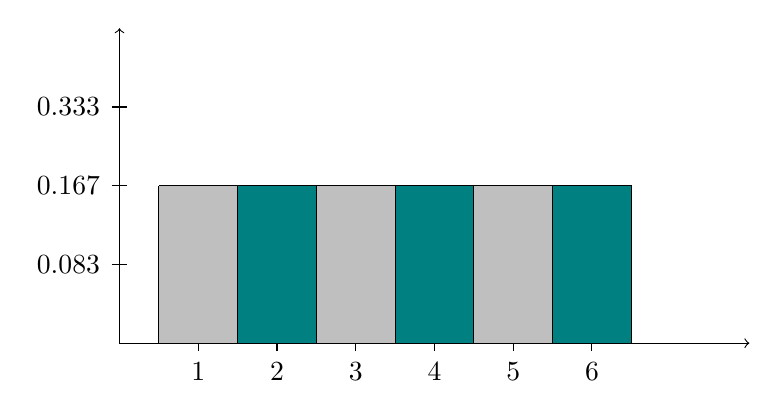
\begin{tikzpicture}

    \draw[->] (0, 0) -- (0, 4);
    \draw (-0.1, 1) -- (0.1, 1);
    \node (ytick1) at (0, 1) [label=left:{0.083}] {};
    \draw (-0.1, 2) -- (0.1, 2);
    \node (ytick2) at (0, 2) [label=left:{0.167}] {};
    \draw (-0.1, 3) -- (0.1, 3);
    \node (ytick3) at (0, 3) [label=left:{0.333}] {};

    \draw[->] (0, 0) -- (8, 0);
    \draw (1, -0.1) -- (1, 0.1);
    \node (xtick1) at (1, 0) [label=below:{1}] {};
    \draw (2, -0.1) -- (2, 0.1);
    \node (xtick2) at (2, 0) [label=below:{2}] {};
    \draw (3, -0.1) -- (3, 0.1);
    \node (xtick3) at (3, 0) [label=below:{3}] {};
    \draw (4, -0.1) -- (4, 0.1);
    \node (xtick4) at (4, 0) [label=below:{4}] {};
    \draw (5, -0.1) -- (5, 0.1);
    \node (xtick5) at (5, 0) [label=below:{5}] {};
    \draw (6, -0.1) -- (6, 0.1);
    \node (xtick6) at (6, 0) [label=below:{6}] {};

    \draw[fill=lightgray] (0.5, 2) -- (6.5, 2) -- (6.5, 0) -- (0.5, 0) -- (0.5, 2);
    \draw (1.5, 2) -- (1.5, 0);
    \draw[fill=teal] (1.5, 2) -- (2.5, 2) -- (2.5, 0) -- (1.5, 0) -- (1.5, 2);
    \draw (3.5, 2) -- (3.5, 0);
    \draw (4.5, 2) -- (4.5, 0);
    \draw[fill=teal] (3.5, 2) -- (4.5, 2) -- (4.5, 0) -- (3.5, 0) -- (3.5, 2); 
    \draw (5.5, 2) -- (5.5, 0);
    \draw[fill=teal] (5.5, 2) -- (6.5, 2) -- (6.5, 0) -- (5.5, 0) -- (5.5, 2);

  \end{tikzpicture}
\end{center}

What's the probability of rolling a number greater than 2? It's four-sixths, or .666:

\begin{center}
  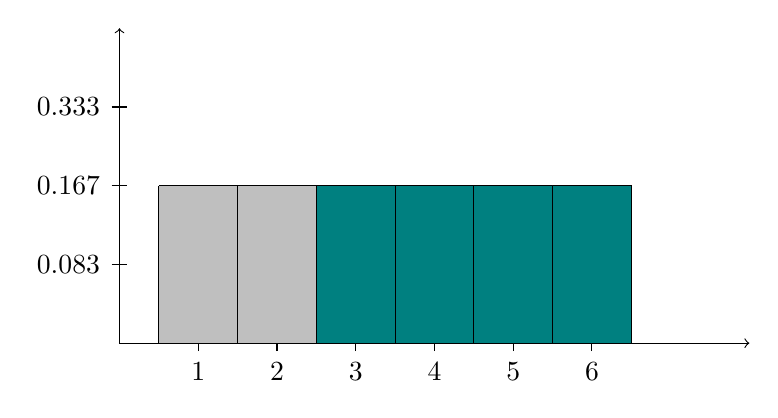
\begin{tikzpicture}

    \draw[->] (0, 0) -- (0, 4);
    \draw (-0.1, 1) -- (0.1, 1);
    \node (ytick1) at (0, 1) [label=left:{0.083}] {};
    \draw (-0.1, 2) -- (0.1, 2);
    \node (ytick2) at (0, 2) [label=left:{0.167}] {};
    \draw (-0.1, 3) -- (0.1, 3);
    \node (ytick3) at (0, 3) [label=left:{0.333}] {};

    \draw[->] (0, 0) -- (8, 0);
    \draw (1, -0.1) -- (1, 0.1);
    \node (xtick1) at (1, 0) [label=below:{1}] {};
    \draw (2, -0.1) -- (2, 0.1);
    \node (xtick2) at (2, 0) [label=below:{2}] {};
    \draw (3, -0.1) -- (3, 0.1);
    \node (xtick3) at (3, 0) [label=below:{3}] {};
    \draw (4, -0.1) -- (4, 0.1);
    \node (xtick4) at (4, 0) [label=below:{4}] {};
    \draw (5, -0.1) -- (5, 0.1);
    \node (xtick5) at (5, 0) [label=below:{5}] {};
    \draw (6, -0.1) -- (6, 0.1);
    \node (xtick6) at (6, 0) [label=below:{6}] {};

    \draw[fill=lightgray] (0.5, 2) -- (6.5, 2) -- (6.5, 0) -- (0.5, 0) -- (0.5, 2);
    \draw (1.5, 2) -- (1.5, 0);
    \draw (3.5, 2) -- (3.5, 0);
    \draw[fill=teal] (2.5, 2) -- (3.5, 2) -- (3.5, 0) -- (2.5, 0) -- (2.5, 2);
    \draw (4.5, 2) -- (4.5, 0);
    \draw[fill=teal] (3.5, 2) -- (4.5, 2) -- (4.5, 0) -- (3.5, 0) -- (3.5, 2); 
    \draw (5.5, 2) -- (5.5, 0);
    \draw[fill=teal] (4.5, 2) -- (5.5, 2) -- (5.5, 0) -- (4.5, 0) -- (4.5, 2); 
    \draw[fill=teal] (5.5, 2) -- (6.5, 2) -- (6.5, 0) -- (5.5, 0) -- (5.5, 2);

  \end{tikzpicture}
\end{center}

What's the probability of rolling a number greater than or equal to 2? It's five-sixths, or 0.833. 

\begin{center}
  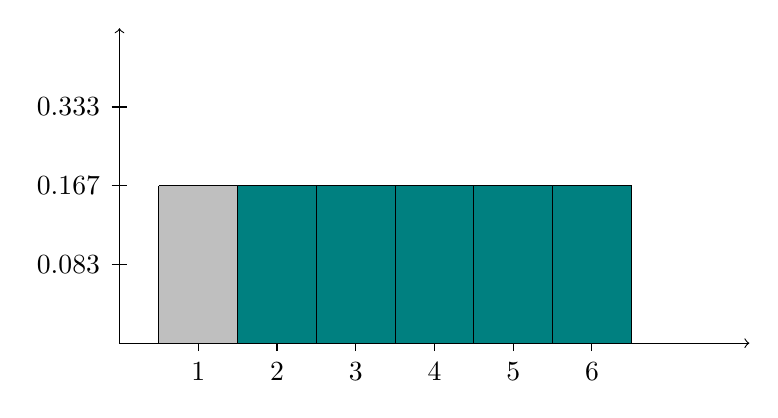
\begin{tikzpicture}

    \draw[->] (0, 0) -- (0, 4);
    \draw (-0.1, 1) -- (0.1, 1);
    \node (ytick1) at (0, 1) [label=left:{0.083}] {};
    \draw (-0.1, 2) -- (0.1, 2);
    \node (ytick2) at (0, 2) [label=left:{0.167}] {};
    \draw (-0.1, 3) -- (0.1, 3);
    \node (ytick3) at (0, 3) [label=left:{0.333}] {};

    \draw[->] (0, 0) -- (8, 0);
    \draw (1, -0.1) -- (1, 0.1);
    \node (xtick1) at (1, 0) [label=below:{1}] {};
    \draw (2, -0.1) -- (2, 0.1);
    \node (xtick2) at (2, 0) [label=below:{2}] {};
    \draw (3, -0.1) -- (3, 0.1);
    \node (xtick3) at (3, 0) [label=below:{3}] {};
    \draw (4, -0.1) -- (4, 0.1);
    \node (xtick4) at (4, 0) [label=below:{4}] {};
    \draw (5, -0.1) -- (5, 0.1);
    \node (xtick5) at (5, 0) [label=below:{5}] {};
    \draw (6, -0.1) -- (6, 0.1);
    \node (xtick6) at (6, 0) [label=below:{6}] {};

    \draw[fill=lightgray] (0.5, 2) -- (6.5, 2) -- (6.5, 0) -- (0.5, 0) -- (0.5, 2);
    \draw (1.5, 2) -- (1.5, 0);
    \draw[fill=teal] (1.5, 2) -- (2.5, 2) -- (2.5, 0) -- (1.5, 0) -- (1.5, 2);
    \draw (3.5, 2) -- (3.5, 0);
    \draw[fill=teal] (2.5, 2) -- (3.5, 2) -- (3.5, 0) -- (2.5, 0) -- (2.5, 2);
    \draw (4.5, 2) -- (4.5, 0);
    \draw[fill=teal] (3.5, 2) -- (4.5, 2) -- (4.5, 0) -- (3.5, 0) -- (3.5, 2); 
    \draw (5.5, 2) -- (5.5, 0);
    \draw[fill=teal] (4.5, 2) -- (5.5, 2) -- (5.5, 0) -- (4.5, 0) -- (4.5, 2); 
    \draw[fill=teal] (5.5, 2) -- (6.5, 2) -- (6.5, 0) -- (5.5, 0) -- (5.5, 2);

  \end{tikzpicture}
\end{center}

What's the probability of rolling a number less than 3? It's two-sixths, or 0.333:

\begin{center}
  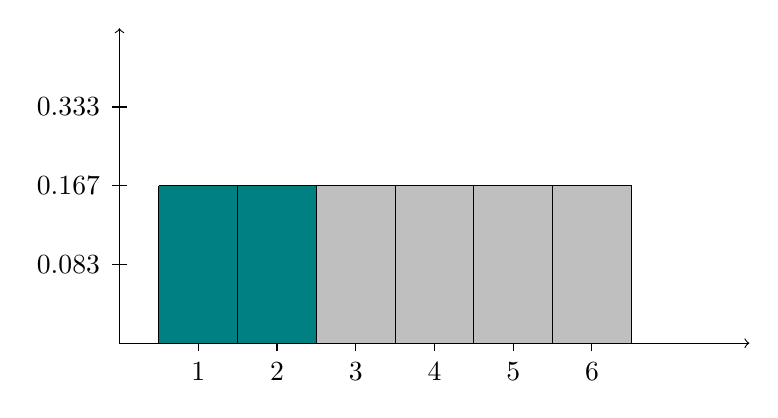
\begin{tikzpicture}

    \draw[->] (0, 0) -- (0, 4);
    \draw (-0.1, 1) -- (0.1, 1);
    \node (ytick1) at (0, 1) [label=left:{0.083}] {};
    \draw (-0.1, 2) -- (0.1, 2);
    \node (ytick2) at (0, 2) [label=left:{0.167}] {};
    \draw (-0.1, 3) -- (0.1, 3);
    \node (ytick3) at (0, 3) [label=left:{0.333}] {};

    \draw[->] (0, 0) -- (8, 0);
    \draw (1, -0.1) -- (1, 0.1);
    \node (xtick1) at (1, 0) [label=below:{1}] {};
    \draw (2, -0.1) -- (2, 0.1);
    \node (xtick2) at (2, 0) [label=below:{2}] {};
    \draw (3, -0.1) -- (3, 0.1);
    \node (xtick3) at (3, 0) [label=below:{3}] {};
    \draw (4, -0.1) -- (4, 0.1);
    \node (xtick4) at (4, 0) [label=below:{4}] {};
    \draw (5, -0.1) -- (5, 0.1);
    \node (xtick5) at (5, 0) [label=below:{5}] {};
    \draw (6, -0.1) -- (6, 0.1);
    \node (xtick6) at (6, 0) [label=below:{6}] {};

    \draw[fill=lightgray] (0.5, 2) -- (6.5, 2) -- (6.5, 0) -- (0.5, 0) -- (0.5, 2);
    \draw[fill=teal] (0.5, 2) -- (1.5, 2) -- (1.5, 0) -- (0.5, 0) -- (0.5, 2);
    \draw (1.5, 2) -- (1.5, 0);
    \draw[fill=teal] (1.5, 2) -- (2.5, 2) -- (2.5, 0) -- (1.5, 0) -- (1.5, 2);
    \draw (3.5, 2) -- (3.5, 0);
    \draw (4.5, 2) -- (4.5, 0);
    \draw (5.5, 2) -- (5.5, 0);

  \end{tikzpicture}
\end{center}

So, we can see a lot about probabilities just by looking at the area that the outcomes take up.


%%%%%%%%%%%%%%%%%%%%%%%%%%%%%%%%%%%%%%%%%
%%%%%%%%%%%%%%%%%%%%%%%%%%%%%%%%%%%%%%%%%
\section{Adding up areas}

In these last examples, we added up the different segments to get the total. In other words, we get a sequence of probabilities, and we accumulate them. This is a useful technique.


%%%%%%%%%%%%%%%%%%%%%%%%%%%%%%%%%%%%%%%%%
\subsection{Example}

Take the distribution of rolling a six-sided die that we plotted above.

Now, we can ask: what is the probability of rolling a number less than 4? Here is the notation:

\begin{equation*}
    \Probability{\RandVarVal/ < 4}
\end{equation*}

\noindent
To compute the answer, we use the \PDFtext/ to get the probability of 0, then 1, then 2, and then 3, and we add them up:

\begin{equation*}
    \Probability{\RandVarVal/ < 4} = \Probability{\RandVarVal/ = 0} + \Probability{\RandVarVal/ = 1} + \Probability{\RandVarVal/ = 2} + \Probability{\RandVarVal/ + 3}
\end{equation*}

\noindent
Which amounts to this:

\begin{equation*}
    \Probability{\RandVarVal/ < 4} = 0.167 + 0.167 + 0.167 + 0.167 = 0.667
\end{equation*}


%%%%%%%%%%%%%%%%%%%%%%%%%%%%%%%%%%%%%%%%%
%%%%%%%%%%%%%%%%%%%%%%%%%%%%%%%%%%%%%%%%%
\subsection{Another example}

Take the same distribution of rolling a six-sided die. What is the probability of rolling a value greater than 2? That is:

\begin{equation*}
  \Probability{\RandVarVal/ > 2}
\end{equation*}

\noindent
We could add up the probability of $\RandVarVal/ = 3$, $\RandVarVal/ = 4$, $\RandVarVal/ = 5$, and $\RandVarVal/ = 6$. But we could also just compute the probability of $\RandVarVal/ = 1$ and $\RandVarVal/ = 2$, and then subtract that from 1. 

After all, we know that the entire probability adds up to 1, and so if we take away the probabilities of $\RandVarVal/ = 1$ and $\RandVarVal/ = 2$, then the remaining area will be the probability of getting \emph{everything} greater than 2:

\begin{equation*}
  \Probability{\RandVarVal/ > 2} = 1 - (\Probability{\RandVarVal/ = 1} + \Probability{\RandVarVal/ = 2})
\end{equation*} 

This is a useful technique. If you want to find the probability of everything \emph{greater} than some value $\RandVarVal/$, calculate the probability of everything below it, and then subtract it from 1. 


%%%%%%%%%%%%%%%%%%%%%%%%%%%%%%%%%%%%%%%%%
%%%%%%%%%%%%%%%%%%%%%%%%%%%%%%%%%%%%%%%%%
\section{Adding more sides to the die}

Okay, so far we've talked about calculating the probability for discrete values by using the area of a polygon plot. But we've been dealing with small numbers of values. In a coin flip, there are only two outcomes, and with a six-sided die, there are only six possible outcomes. 

Let's start making the number of outcomes bigger. Think of rolling a (fair) die with many more sides. Say, 10 sides. 

\begin{center}
  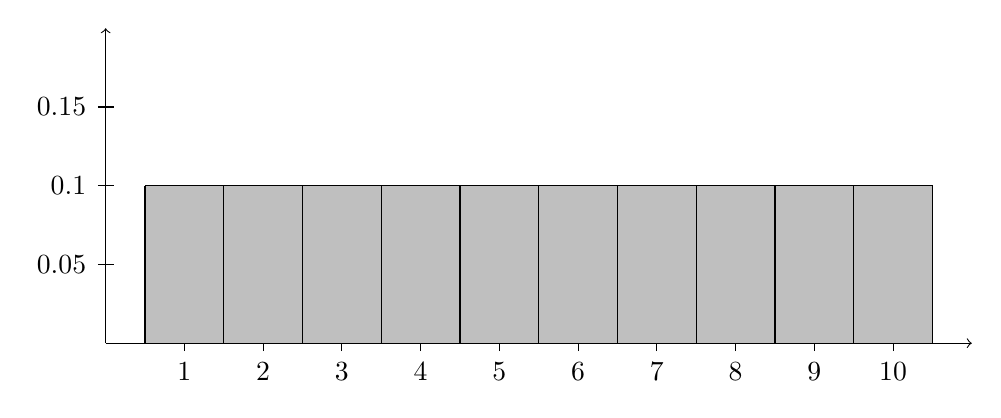
\begin{tikzpicture}

    \draw[->] (0, 0) -- (0, 4);
    \draw (-0.1, 1) -- (0.1, 1);
    \node (ytick1) at (0, 1) [label=left:{0.05}] {};
    \draw (-0.1, 2) -- (0.1, 2);
    \node (ytick2) at (0, 2) [label=left:{0.1}] {};
    \draw (-0.1, 3) -- (0.1, 3);
    \node (ytick3) at (0, 3) [label=left:{0.15}] {};

    \draw[->] (0, 0) -- (11, 0);
    \draw (1, -0.1) -- (1, 0.1);
    \node (xtick1) at (1, 0) [label=below:{1}] {};
    \draw (2, -0.1) -- (2, 0.1);
    \node (xtick2) at (2, 0) [label=below:{2}] {};
    \draw (3, -0.1) -- (3, 0.1);
    \node (xtick3) at (3, 0) [label=below:{3}] {};
    \draw (4, -0.1) -- (4, 0.1);
    \node (xtick4) at (4, 0) [label=below:{4}] {};
    \draw (5, -0.1) -- (5, 0.1);
    \node (xtick5) at (5, 0) [label=below:{5}] {};
    \draw (6, -0.1) -- (6, 0.1);
    \node (xtick6) at (6, 0) [label=below:{6}] {};
    \draw (7, -0.1) -- (7, 0.1);
    \node (xtick7) at (7, 0) [label=below:{7}] {};
    \draw (8, -0.1) -- (8, 0.1);
    \node (xtick8) at (8, 0) [label=below:{8}] {};
    \draw (9, -0.1) -- (9, 0.1);
    \node (xtick9) at (9, 0) [label=below:{9}] {};
    \draw (10, -0.1) -- (10, 0.1);
    \node (xtick10) at (10, 0) [label=below:{10}] {};

    \draw[fill=lightgray] (0.5, 2) -- (10.5, 2) -- (10.5, 0) -- (0.5, 0) -- (0.5, 2);
    \draw (1.5, 2) -- (1.5, 0);
    \draw (2.5, 2) -- (2.5, 0);
    \draw (3.5, 2) -- (3.5, 0);
    \draw (4.5, 2) -- (4.5, 0);
    \draw (5.5, 2) -- (5.5, 0);
    \draw (6.5, 2) -- (6.5, 0);
    \draw (7.5, 2) -- (7.5, 0);
    \draw (8.5, 2) -- (8.5, 0);
    \draw (9.5, 2) -- (9.5, 0);

  \end{tikzpicture}
\end{center}

Here too, the area of each segment is exactly one-tenth of the whole, and that exactly represents the probability for each outcome. But since we have to fit more segments into the square, we have skinnier segments. And it's even harder now to throw a dart at the plot and hit a particular segment.

Now imagine that we have a (fair) die with, say, 100 sides. The plot would again be a square, but broken up into 100 segments. The area of each segment would be exactly one one-hundredth of the whole, which again exactly represents the probability for each outcome. But the segments would be quite skinny, because now we have to fit 100 of them into the square. And now it's really hard to throw a dart at the plot and hit a particular segment. The segments are just too skinny.

Think about a (fair) die with, say, a million sides. Now the segments would be extremely skinny, and hitting any particular segment with a dart is practically impossible. The segments are way too skinny to even tell them apart.

And imagine that we break the square up into an infinite number of segments. These segments are so small they're just slivers with no width at all! It's just an infinite number of slivers packed into the square.

This helps to visualize the idea that, once we have an infinite number of slivers packed into that square, the probability of hitting any particular sliver is just zero, or nil.



%%%%%%%%%%%%%%%%%%%%%%%%%%%%%%%%%%%%%%%%%
%%%%%%%%%%%%%%%%%%%%%%%%%%%%%%%%%%%%%%%%%
\section{Probability is just the area}

So, for continuous values, if the probability of any particular outcome is zero, how the heck do we calculate the probability of an outcome? 

The answer is that we measure the probability of falling somewhere inside a \vocab{range}. 

\begin{itemize}
  \item So we don't look for the probability of exactly (say) 3.015 grams. 
  \item Instead, we look for the probability of being somewhere in between (say) 3 and 3.5 grams.
\end{itemize}

\noindent
With discrete values, the function we use to pair up outcomes with probabilities is called a \vocab{probability distribution function}, or \PDFtext/ for short. When we are dealing with continuous values, however, we are working not with discrete values, but rather with areas. So we have a different name for the distribution functions that we use for continuous values. We call them \vocab{cumulative distribution functions}, or \CDFtext/s for short. So:

\begin{itemize}
  \item With discrete values, we call them \PDFtext/s.
  \item With continuous values, we call them \CDFtext/s.
\end{itemize}



\end{document}
